% Options for packages loaded elsewhere
\PassOptionsToPackage{unicode}{hyperref}
\PassOptionsToPackage{hyphens}{url}
%
\documentclass[
  ignorenonframetext,
]{beamer}
\usepackage{pgfpages}
\setbeamertemplate{caption}[numbered]
\setbeamertemplate{caption label separator}{: }
\setbeamercolor{caption name}{fg=normal text.fg}
\beamertemplatenavigationsymbolsempty
% Prevent slide breaks in the middle of a paragraph
\widowpenalties 1 10000
\raggedbottom
\setbeamertemplate{part page}{
  \centering
  \begin{beamercolorbox}[sep=16pt,center]{part title}
    \usebeamerfont{part title}\insertpart\par
  \end{beamercolorbox}
}
\setbeamertemplate{section page}{
  \centering
  \begin{beamercolorbox}[sep=12pt,center]{part title}
    \usebeamerfont{section title}\insertsection\par
  \end{beamercolorbox}
}
\setbeamertemplate{subsection page}{
  \centering
  \begin{beamercolorbox}[sep=8pt,center]{part title}
    \usebeamerfont{subsection title}\insertsubsection\par
  \end{beamercolorbox}
}
\AtBeginPart{
  \frame{\partpage}
}
\AtBeginSection{
  \ifbibliography
  \else
    \frame{\sectionpage}
  \fi
}
\AtBeginSubsection{
  \frame{\subsectionpage}
}
\usepackage{amsmath,amssymb}
\usepackage{lmodern}
\usepackage{ifxetex,ifluatex}
\ifnum 0\ifxetex 1\fi\ifluatex 1\fi=0 % if pdftex
  \usepackage[T1]{fontenc}
  \usepackage[utf8]{inputenc}
  \usepackage{textcomp} % provide euro and other symbols
\else % if luatex or xetex
  \usepackage{unicode-math}
  \defaultfontfeatures{Scale=MatchLowercase}
  \defaultfontfeatures[\rmfamily]{Ligatures=TeX,Scale=1}
\fi
\usetheme[]{Antibes}
\usefonttheme{structurebold}
% Use upquote if available, for straight quotes in verbatim environments
\IfFileExists{upquote.sty}{\usepackage{upquote}}{}
\IfFileExists{microtype.sty}{% use microtype if available
  \usepackage[]{microtype}
  \UseMicrotypeSet[protrusion]{basicmath} % disable protrusion for tt fonts
}{}
\makeatletter
\@ifundefined{KOMAClassName}{% if non-KOMA class
  \IfFileExists{parskip.sty}{%
    \usepackage{parskip}
  }{% else
    \setlength{\parindent}{0pt}
    \setlength{\parskip}{6pt plus 2pt minus 1pt}}
}{% if KOMA class
  \KOMAoptions{parskip=half}}
\makeatother
\usepackage{xcolor}
\IfFileExists{xurl.sty}{\usepackage{xurl}}{} % add URL line breaks if available
\IfFileExists{bookmark.sty}{\usepackage{bookmark}}{\usepackage{hyperref}}
\hypersetup{
  pdftitle={Title here},
  pdfauthor={Christian Coffman},
  hidelinks,
  pdfcreator={LaTeX via pandoc}}
\urlstyle{same} % disable monospaced font for URLs
\newif\ifbibliography
\usepackage{color}
\usepackage{fancyvrb}
\newcommand{\VerbBar}{|}
\newcommand{\VERB}{\Verb[commandchars=\\\{\}]}
\DefineVerbatimEnvironment{Highlighting}{Verbatim}{commandchars=\\\{\}}
% Add ',fontsize=\small' for more characters per line
\usepackage{framed}
\definecolor{shadecolor}{RGB}{248,248,248}
\newenvironment{Shaded}{\begin{snugshade}}{\end{snugshade}}
\newcommand{\AlertTok}[1]{\textcolor[rgb]{0.94,0.16,0.16}{#1}}
\newcommand{\AnnotationTok}[1]{\textcolor[rgb]{0.56,0.35,0.01}{\textbf{\textit{#1}}}}
\newcommand{\AttributeTok}[1]{\textcolor[rgb]{0.77,0.63,0.00}{#1}}
\newcommand{\BaseNTok}[1]{\textcolor[rgb]{0.00,0.00,0.81}{#1}}
\newcommand{\BuiltInTok}[1]{#1}
\newcommand{\CharTok}[1]{\textcolor[rgb]{0.31,0.60,0.02}{#1}}
\newcommand{\CommentTok}[1]{\textcolor[rgb]{0.56,0.35,0.01}{\textit{#1}}}
\newcommand{\CommentVarTok}[1]{\textcolor[rgb]{0.56,0.35,0.01}{\textbf{\textit{#1}}}}
\newcommand{\ConstantTok}[1]{\textcolor[rgb]{0.00,0.00,0.00}{#1}}
\newcommand{\ControlFlowTok}[1]{\textcolor[rgb]{0.13,0.29,0.53}{\textbf{#1}}}
\newcommand{\DataTypeTok}[1]{\textcolor[rgb]{0.13,0.29,0.53}{#1}}
\newcommand{\DecValTok}[1]{\textcolor[rgb]{0.00,0.00,0.81}{#1}}
\newcommand{\DocumentationTok}[1]{\textcolor[rgb]{0.56,0.35,0.01}{\textbf{\textit{#1}}}}
\newcommand{\ErrorTok}[1]{\textcolor[rgb]{0.64,0.00,0.00}{\textbf{#1}}}
\newcommand{\ExtensionTok}[1]{#1}
\newcommand{\FloatTok}[1]{\textcolor[rgb]{0.00,0.00,0.81}{#1}}
\newcommand{\FunctionTok}[1]{\textcolor[rgb]{0.00,0.00,0.00}{#1}}
\newcommand{\ImportTok}[1]{#1}
\newcommand{\InformationTok}[1]{\textcolor[rgb]{0.56,0.35,0.01}{\textbf{\textit{#1}}}}
\newcommand{\KeywordTok}[1]{\textcolor[rgb]{0.13,0.29,0.53}{\textbf{#1}}}
\newcommand{\NormalTok}[1]{#1}
\newcommand{\OperatorTok}[1]{\textcolor[rgb]{0.81,0.36,0.00}{\textbf{#1}}}
\newcommand{\OtherTok}[1]{\textcolor[rgb]{0.56,0.35,0.01}{#1}}
\newcommand{\PreprocessorTok}[1]{\textcolor[rgb]{0.56,0.35,0.01}{\textit{#1}}}
\newcommand{\RegionMarkerTok}[1]{#1}
\newcommand{\SpecialCharTok}[1]{\textcolor[rgb]{0.00,0.00,0.00}{#1}}
\newcommand{\SpecialStringTok}[1]{\textcolor[rgb]{0.31,0.60,0.02}{#1}}
\newcommand{\StringTok}[1]{\textcolor[rgb]{0.31,0.60,0.02}{#1}}
\newcommand{\VariableTok}[1]{\textcolor[rgb]{0.00,0.00,0.00}{#1}}
\newcommand{\VerbatimStringTok}[1]{\textcolor[rgb]{0.31,0.60,0.02}{#1}}
\newcommand{\WarningTok}[1]{\textcolor[rgb]{0.56,0.35,0.01}{\textbf{\textit{#1}}}}
\usepackage{graphicx}
\makeatletter
\def\maxwidth{\ifdim\Gin@nat@width>\linewidth\linewidth\else\Gin@nat@width\fi}
\def\maxheight{\ifdim\Gin@nat@height>\textheight\textheight\else\Gin@nat@height\fi}
\makeatother
% Scale images if necessary, so that they will not overflow the page
% margins by default, and it is still possible to overwrite the defaults
% using explicit options in \includegraphics[width, height, ...]{}
\setkeys{Gin}{width=\maxwidth,height=\maxheight,keepaspectratio}
% Set default figure placement to htbp
\makeatletter
\def\fps@figure{htbp}
\makeatother
\setlength{\emergencystretch}{3em} % prevent overfull lines
\providecommand{\tightlist}{%
  \setlength{\itemsep}{0pt}\setlength{\parskip}{0pt}}
\setcounter{secnumdepth}{-\maxdimen} % remove section numbering
\definecolor{Gold}{RGB}{255, 204, 51}
\definecolor{Maroon1}{RGB}{112, 0, 25}
\definecolor{Maroon2}{RGB}{92, 0, 15}
\definecolor{Maroon3}{RGB}{92, 0, 15}
\definecolor{Maroon4}{RGB}{82, 0, 10}
\setbeamercolor{palette primary}{bg=Maroon1, fg = Gold}
\setbeamercolor{palette secondary}{bg=Maroon2, fg = Gold}
\setbeamercolor{palette tertiary}{bg=Maroon3, fg = Gold}
\setbeamercolor{palette quaternary}{bg=Maroon4, fg = Gold}
\setbeamercolor{palette sidebar secondary}{bg=Maroon1, fg = Gold}
\setbeamercolor{palette sidebar secondary}{bg=Maroon2, fg = Gold}
\setbeamercolor{palette sidebar tertiary}{bg=Maroon3, fg = Gold}
\setbeamercolor{palette sidebar quaternary}{bg=Maroon4, fg = Gold}
\setbeamercolor{item}{fg = Maroon1}
\ifluatex
  \usepackage{selnolig}  % disable illegal ligatures
\fi
\newlength{\cslhangindent}
\setlength{\cslhangindent}{1.5em}
\newlength{\csllabelwidth}
\setlength{\csllabelwidth}{3em}
\newenvironment{CSLReferences}[2] % #1 hanging-ident, #2 entry spacing
 {% don't indent paragraphs
  \setlength{\parindent}{0pt}
  % turn on hanging indent if param 1 is 1
  \ifodd #1 \everypar{\setlength{\hangindent}{\cslhangindent}}\ignorespaces\fi
  % set entry spacing
  \ifnum #2 > 0
  \setlength{\parskip}{#2\baselineskip}
  \fi
 }%
 {}
\usepackage{calc}
\newcommand{\CSLBlock}[1]{#1\hfill\break}
\newcommand{\CSLLeftMargin}[1]{\parbox[t]{\csllabelwidth}{#1}}
\newcommand{\CSLRightInline}[1]{\parbox[t]{\linewidth - \csllabelwidth}{#1}\break}
\newcommand{\CSLIndent}[1]{\hspace{\cslhangindent}#1}

\title{AdjHE: An efficient way to estimate heritability}
\author{Christian Coffman}
\date{\today \newline \newline 
\includegraphics[width=1.5in,height=\textheight]{/home/christian/Documents/Templates/U_of_m_logos_updated_2021/Goldy Gopher/Goldy-Word-ppt-PNG/color/goldyM2out-RGB.png}}
\institute{Advised by: Dr. Saonli Basu \newline University of Minnesota Twin Cities \newline Division of
Biostatistics}


\AtBeginSection[]{
%  \begin{frame}
%  \vfill
%  \centering
%  \begin{beamercolorbox}[sep=8pt,center,shadow=true,rounded=true]{title}
%    \usebeamerfont{title}\insertsectionhead\par%
%  \end{beamercolorbox}
%  \vfill
%  \end{frame}
}

% Define file path
% \usepackage{import}

\begin{document}
\frame{\titlepage}

\begin{frame}[allowframebreaks]
  \tableofcontents[hideallsubsections]
\end{frame}
\hypertarget{first-section}%


\section{General trait influencers}\label{sec:impact_trait}}
\begin{frame}{General influences on traits}
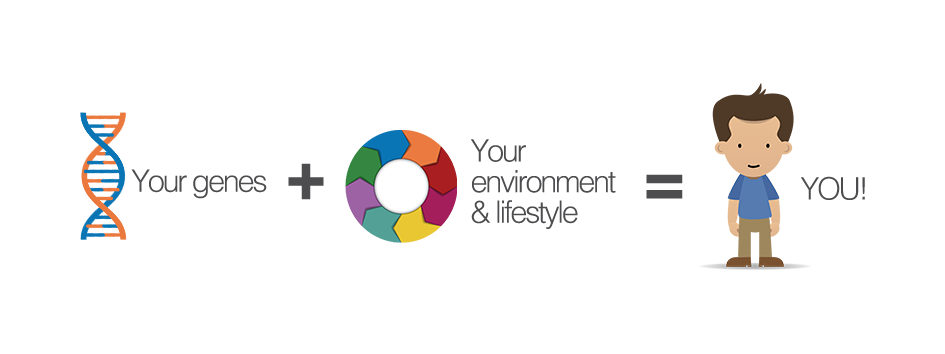
\includegraphics[width = \textwidth]{/home/christian/Research/Stat_gen/tools/Basu_herit/docs/Figures/Introduction/GenesxEnvironment.png} \\
Traits are determined by different contributions of genetics and environmental influencers.\\
Which traits are dictated by which set of influencers?\\
\begin{tiny}
Image credit: https://blogs.kcl.ac.uk/editlab/2019/05/07/if-something-is-genetic-it-can-still-be-influenced-by-the-environment/
\end{tiny}
\end{frame}


\section{Methods for detecting role of genetics}

\begin{frame}{GWAS}
\begin{itemize}
	\item Genome Wide Association studies (GWAS)
	$$Y' = X_c\alpha + X_g\beta + \epsilon $$
	\item $X_g$: genotype
	\item $X_c$: other covariates
	\item Inference done on the $\beta$ (sometimes millions)
	\item Pro: Great for highly influential SNP's
	\item Low: Low power for causality spread across multiple SNP's
\end{itemize}
\end{frame}

\begin{frame}{Gene effects as random}
\begin{itemize}
	\item Consider $\beta \sim N(0, \sigma_g^2 I)$
	\item Then $X_g\beta \sim N(0, \sigma_g^2 X_gX_g')$
	\item Redefined as $N(0, \sigma^2_G A)$
	\item Where A is called the \textbf{Genetic Relatedness Matrix}
	\item Model becomes
	$$Y' = X_c\alpha + \epsilon, \epsilon \sim (0, \sigma_G^2 A + \sigma_e^2I) $$
\end{itemize}

\end{frame}


\begin{frame}{GRM based heritability estimation}
\begin{itemize}
	\item Describe variation in phenotype as random effect (LMM)
		$$ Y' = X_c\alpha + \epsilon, \epsilon \sim N(0, \sigma_g^2 A + \sigma_e^2 I)$$
	\item Gain: power for dispersed genetic effects
	\item Loss: resolution on genome
	\item GCTA uses REML which can be slow with large studies (n x n matrix)
	\item Not efficient for exploration of mildly heritable traits (large sample sizes)
	\item Can solve via MOM, but what about when there is population substructure?
\end{itemize}
\end{frame}

\begin{frame}{New tool: AdjHE}
	\begin{itemize}
		\item Two-stage Method of Moments approach
		\item Accounts for ethnicity as PC's of GRM
		\item Key assumption: $X_c \perp PC's$
		\item Closed form $\therefore$ Much more efficient 
		\item Benchmarked: ~2x faster with 4000 subjects
		\item 10x faster with 45k subjects
	\end{itemize}
	 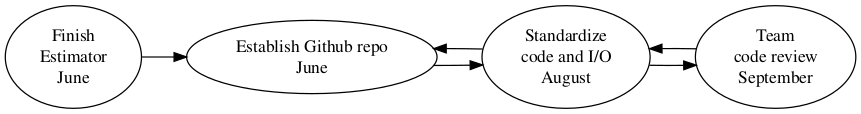
\includegraphics[width = \textwidth]{/home/christian/Research/Stat_gen/tools/Basu_herit/docs/Figures/Diagrams/timeline_diagram.png}
\end{frame}



\begin{frame}{Dealing with population substructure}
\begin{itemize}
	\item Relatedness has family relations $A$ and ethnicity $G$
	$$ GRM = A + G$$
	\begin{center}
		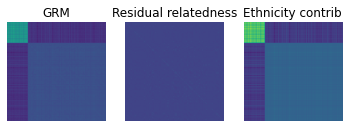
\includegraphics[width = 0.7\textwidth]{/home/christian/Research/Stat_gen/tools/Basu_herit/docs/Figures/Matrices/GRM_decomp.png}
	\end{center}
	\item PCA on GRM
	$$GRM = \sum \lambda_i VV' = \sum \lambda_i A_iA_i' + \sum \lambda_i G_iG_i' $$
	\item Suppose $G_i$ contribute more to variance
	\item First k PC's define G
\end{itemize}
\end{frame}

\begin{frame}{Dealing with covariates}
\begin{itemize}
	\item Treat PC's as covariates ($X = [X_c, X_{pc}]$)
	\item Project away covariates ("Residualize")
	$$ Q = I - X(X'X)^{-1}X' $$
	$$ QY'= Y = QX_c + Q\epsilon = Q\epsilon $$
	$$ EY = 0$$ 
	\item 2nd moment
	$$ EYY' = Var(Y) = Q Var(\epsilon) Q $$
	$$ = \sigma_G^2 A + \sum \delta_i G_iG_i'+ \sigma_e^2 I$$
	\item Solve via OLS
\end{itemize}
\end{frame}

\begin{frame}{Properties of OLS estimator}
$$EYY' = \begin{bmatrix}
A & G_1G_1' & \vdots & G_kG_k' & I 
\end{bmatrix} \begin{bmatrix}
\sigma_G^2 \\ \delta_1 \\ \dots \\ \delta_k \\ \sigma_e^2
\end{bmatrix} $$
$$EYY' - G\delta = \begin{bmatrix}
A & I
\end{bmatrix}
\begin{bmatrix}
\sigma_G^2 \\ \sigma_e^2
\end{bmatrix} $$
$$\begin{bmatrix}
\hat\sigma_G^2 \\ \hat \sigma_e^2
\end{bmatrix} = \begin{bmatrix}
A & I 
\end{bmatrix}
(\begin{bmatrix}
trA^2 & trA \\
trA & n  
\end{bmatrix})^{-1}
\begin{bmatrix}
A \\ I 
\end{bmatrix}(YY' - G\hat \delta)$$
\end{frame}


\begin{frame}{Problem with multi-site estimation}
\begin{itemize}
	\item More studies using consortia to study smaller effects
	\item The Adolescent Brain Cognitive Development (ABCD) has +10,000 subjects > 20 sites
	\item Measures brain features
	\item Brain features sensitive to machine used (i.e. depends on site)
	\item Adding fixed effect blows up SE (coming up in a few slides)
	\item So treat it as random effect
	$$Y \sim N(X_c\alpha, \sigma_G^2A + \sum G_i\delta_i + S\sigma_s^2 + I\sigma_e^2) $$
\end{itemize}
\end{frame}

\begin{frame}{AdjHE site extension}
\begin{itemize}
	\item Assume $X_c \perp X_s, A, G$
	$$	EYY' - G\Delta G' = 
	\begin{bmatrix}
	A & QSQ & I
	\end{bmatrix}\begin{bmatrix}
	\sigma_G^2 \\ \sigma_s^2 \\ \sigma_e^2
	\end{bmatrix}$$
	\item $X_s$ is site vector
	\item $S$ is site similarity matrix $X_sX_s'$
	\end{itemize}
\end{frame}


\section{Simulations}
\begin{frame}{Simulation tool}
\begin{columns}
\begin{column}{0.7\textwidth}
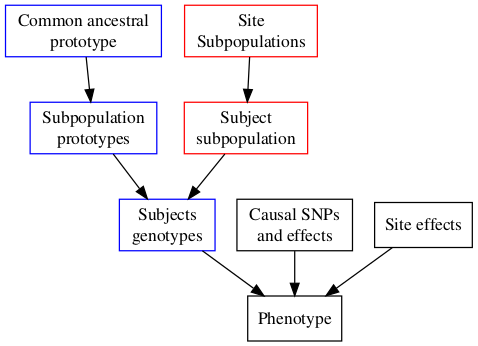
\includegraphics[width = \textwidth]{/home/christian/Research/Stat_gen/tools/Basu_herit/docs/Figures/Diagrams/Simulation_diagram.png}
\end{column}
\begin{column}{0.3\textwidth}
\begin{itemize}
	\item Simulate realistically structured GRM's and phenotypes
	\item Determine what scenarios fit within AdjHE model
\end{itemize}
\end{column}
\end{columns}
\end{frame}


\begin{frame}{Simulating population structures}
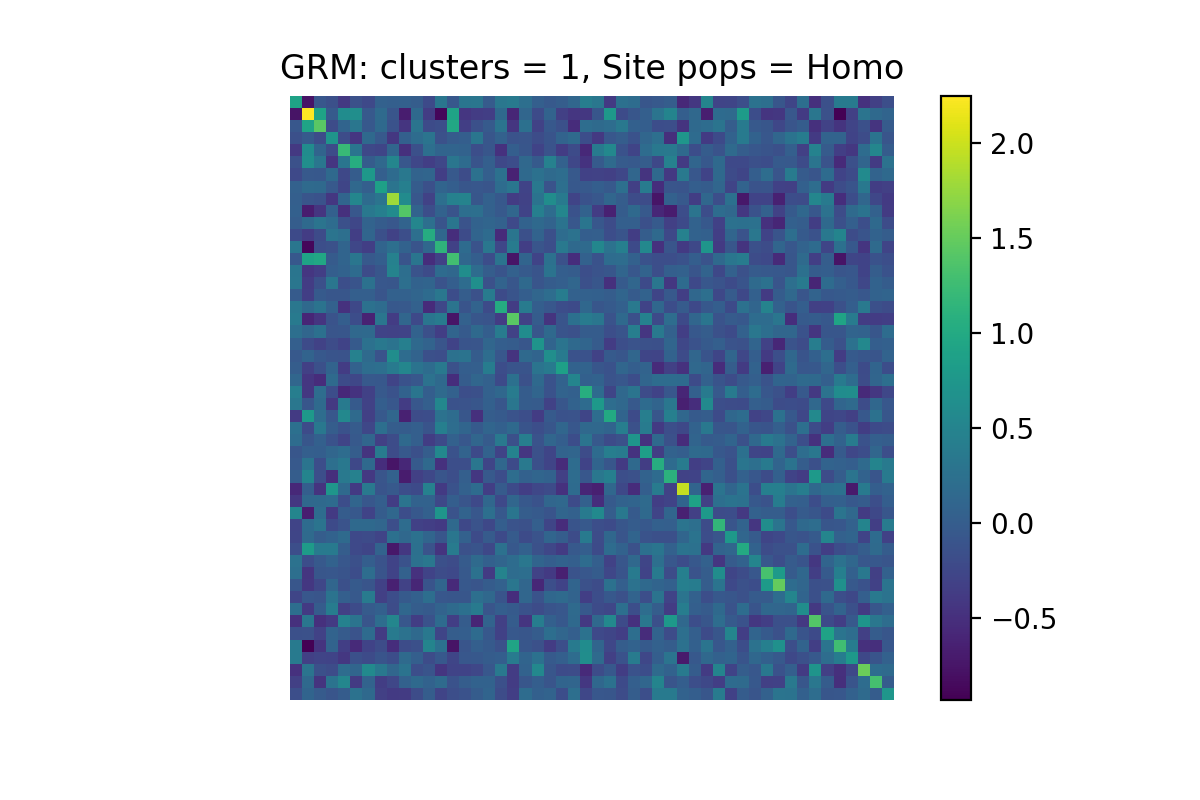
\includegraphics[trim=3cm 0cm 3cm 0cm, clip,width = 0.49\textwidth]{/home/christian/Research/Stat_gen/tools/Basu_herit/docs/Figures/Matrices/GRM_50_10_1_Homo.png}
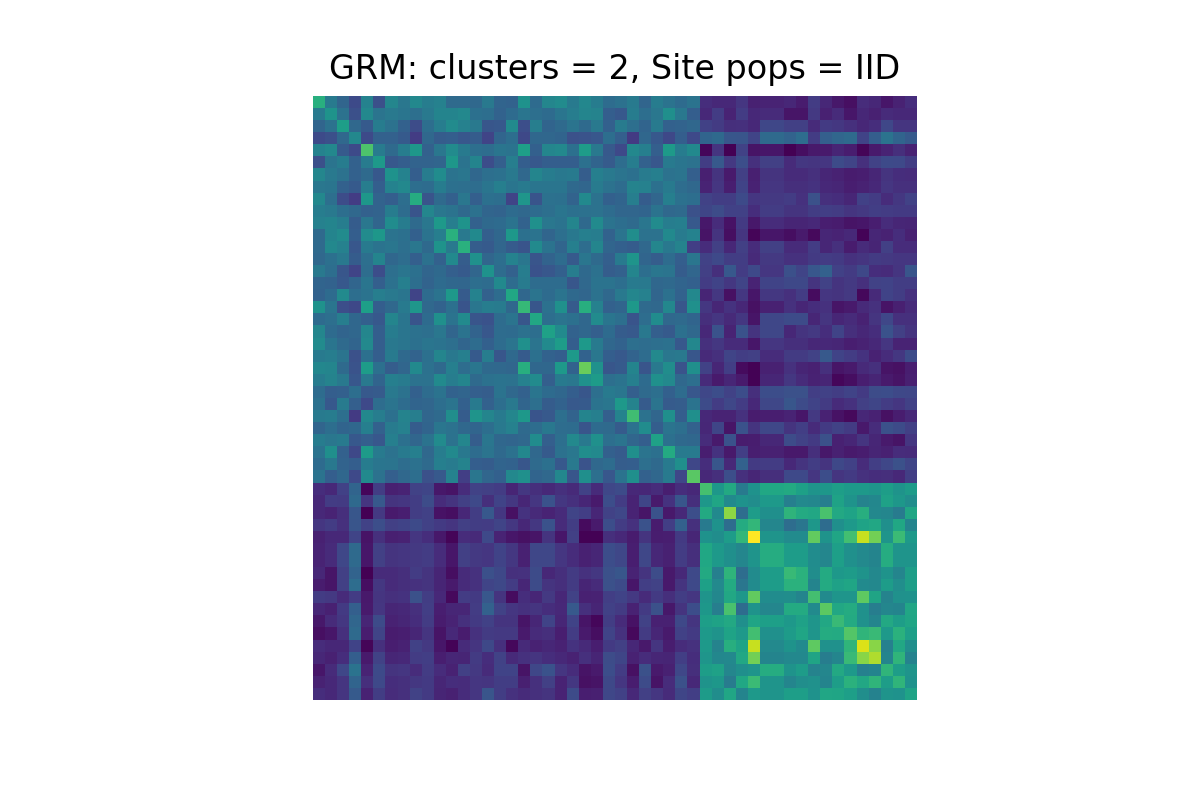
\includegraphics[trim=3cm 0cm 3cm 0cm, clip,width = 0.49\textwidth]{/home/christian/Research/Stat_gen/tools/Basu_herit/docs/Figures/Matrices/GRM_50_10_2_IID.png}
\end{frame}


\begin{frame}{Estimation on Homogeneous}
\centering
 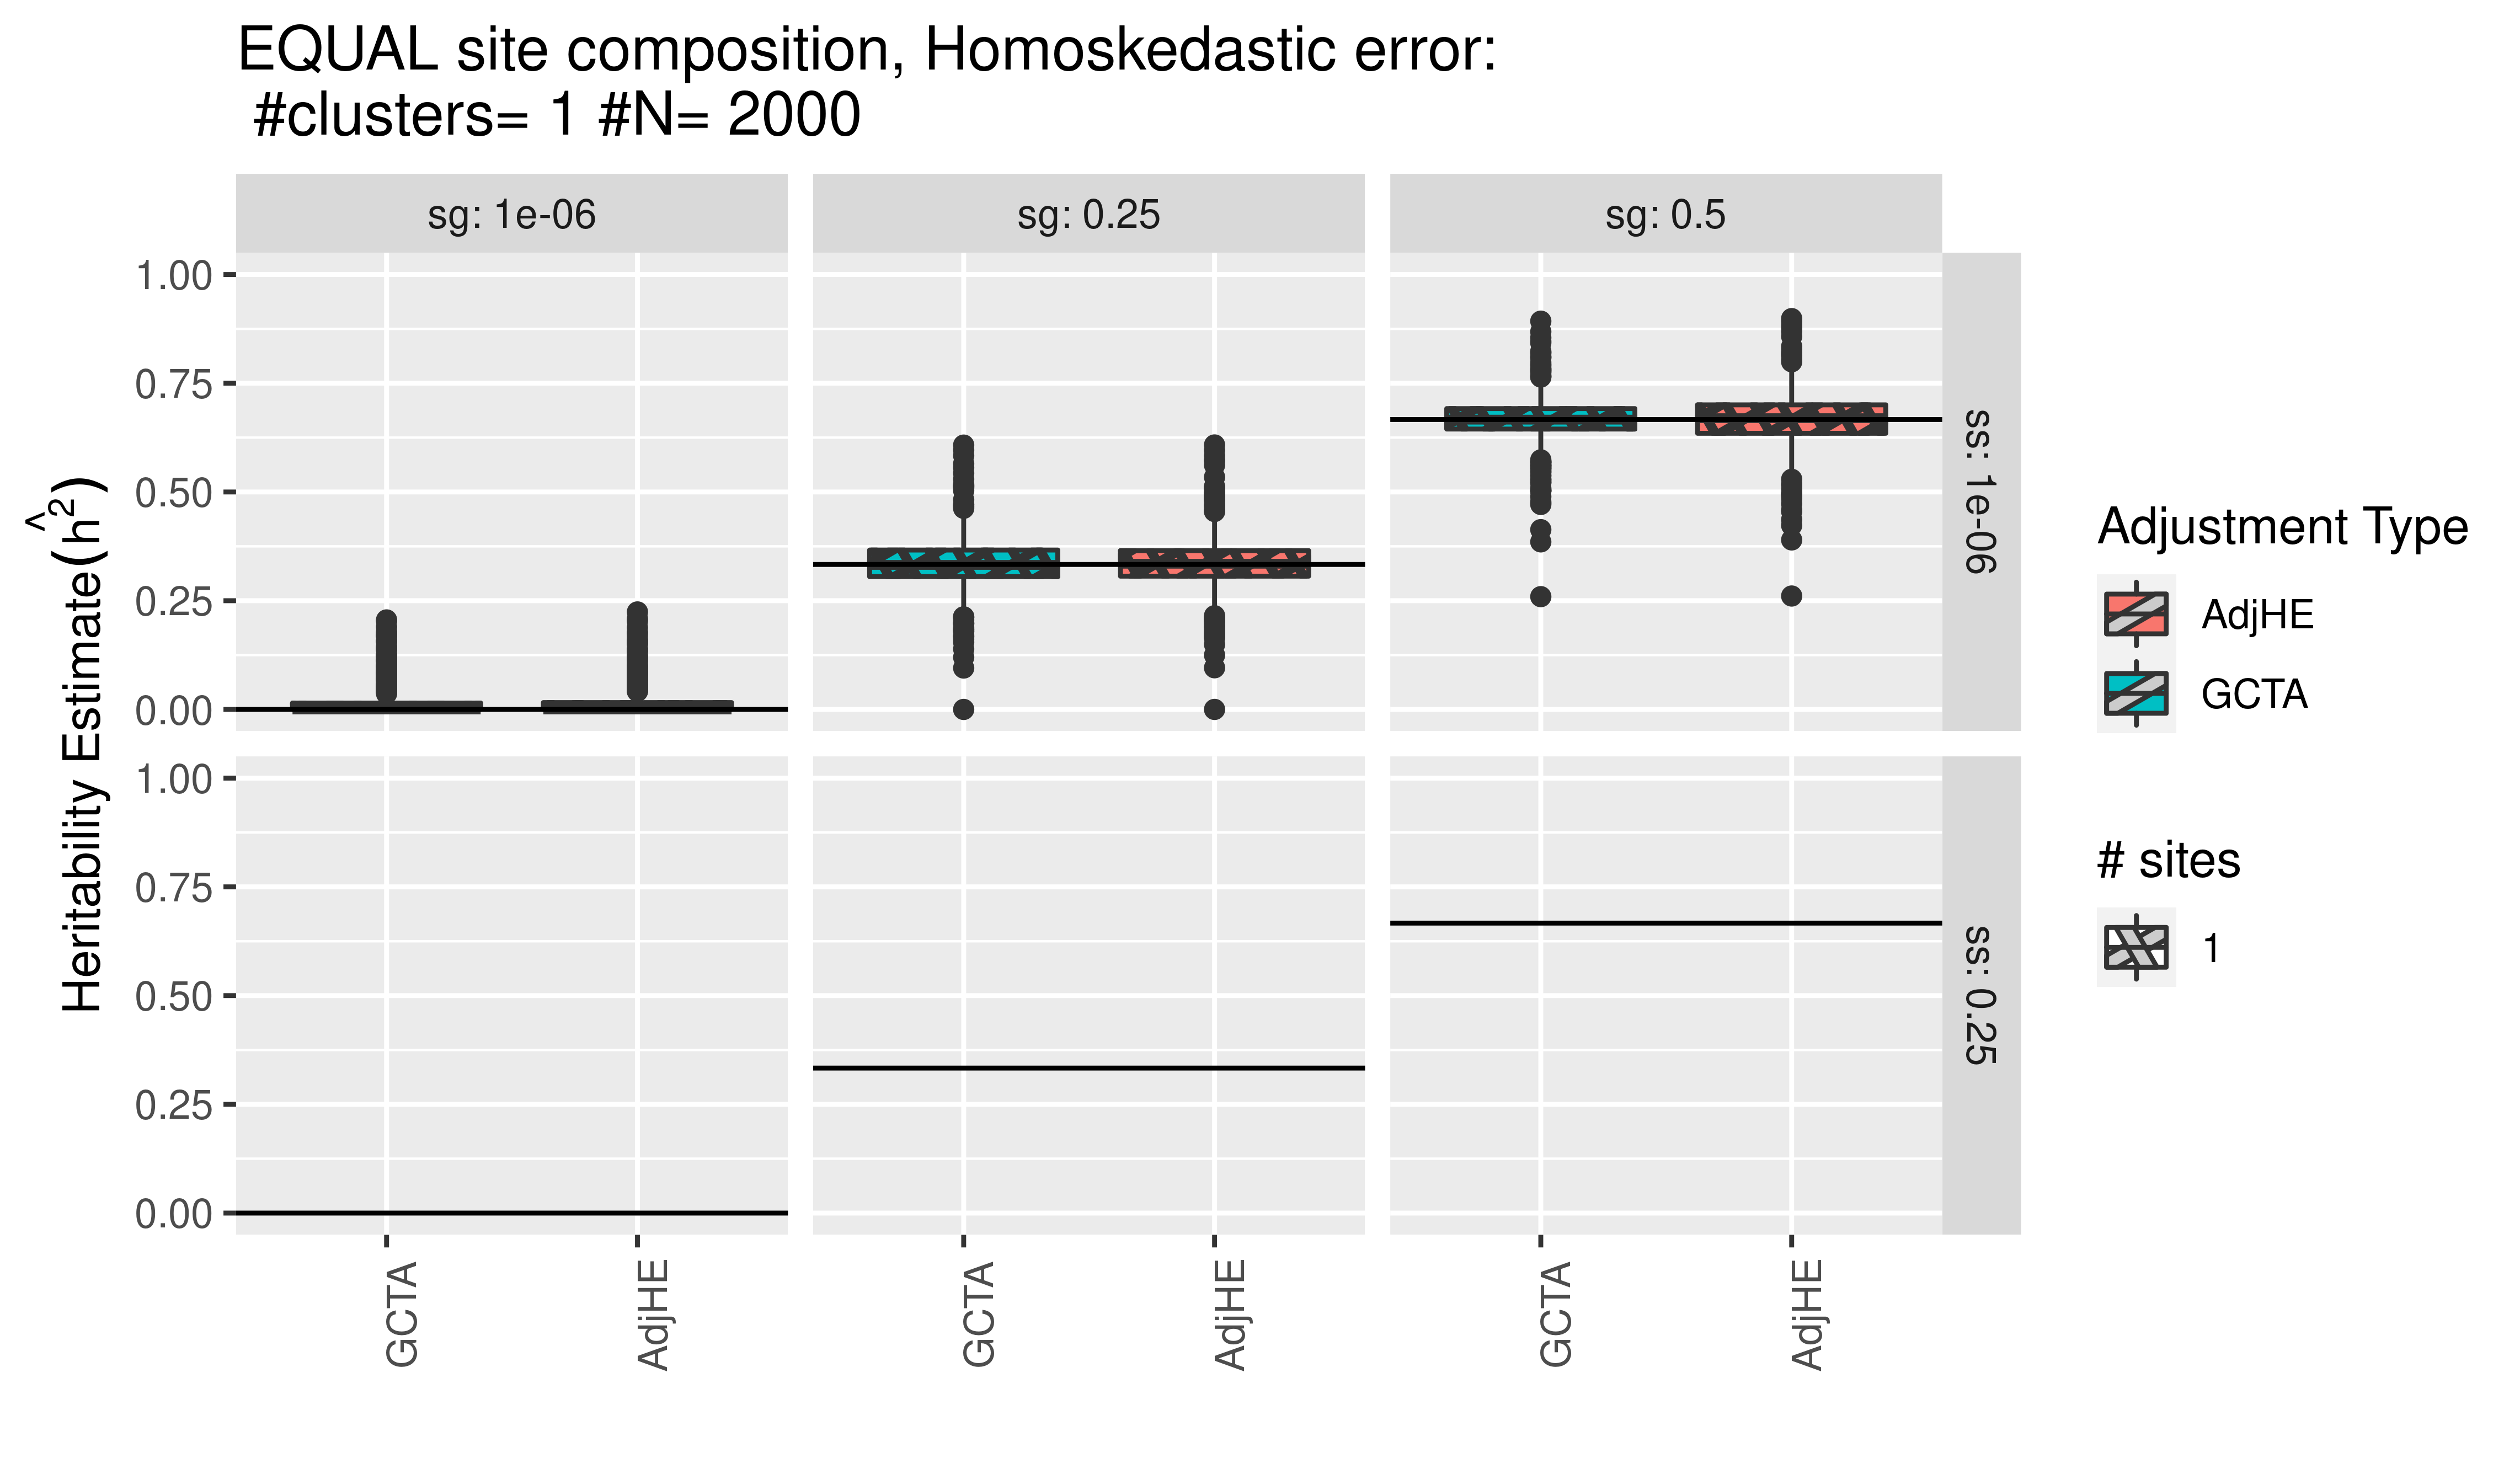
\includegraphics[width = 1.2\textwidth]{/home/christian/Research/Stat_gen/tools/Basu_herit/docs/Figures/Estimates/Simulations/N2000_C1_EQUAL_Homo.png}
\end{frame}

\begin{frame}{Estimation on Homogeneous}
\centering
 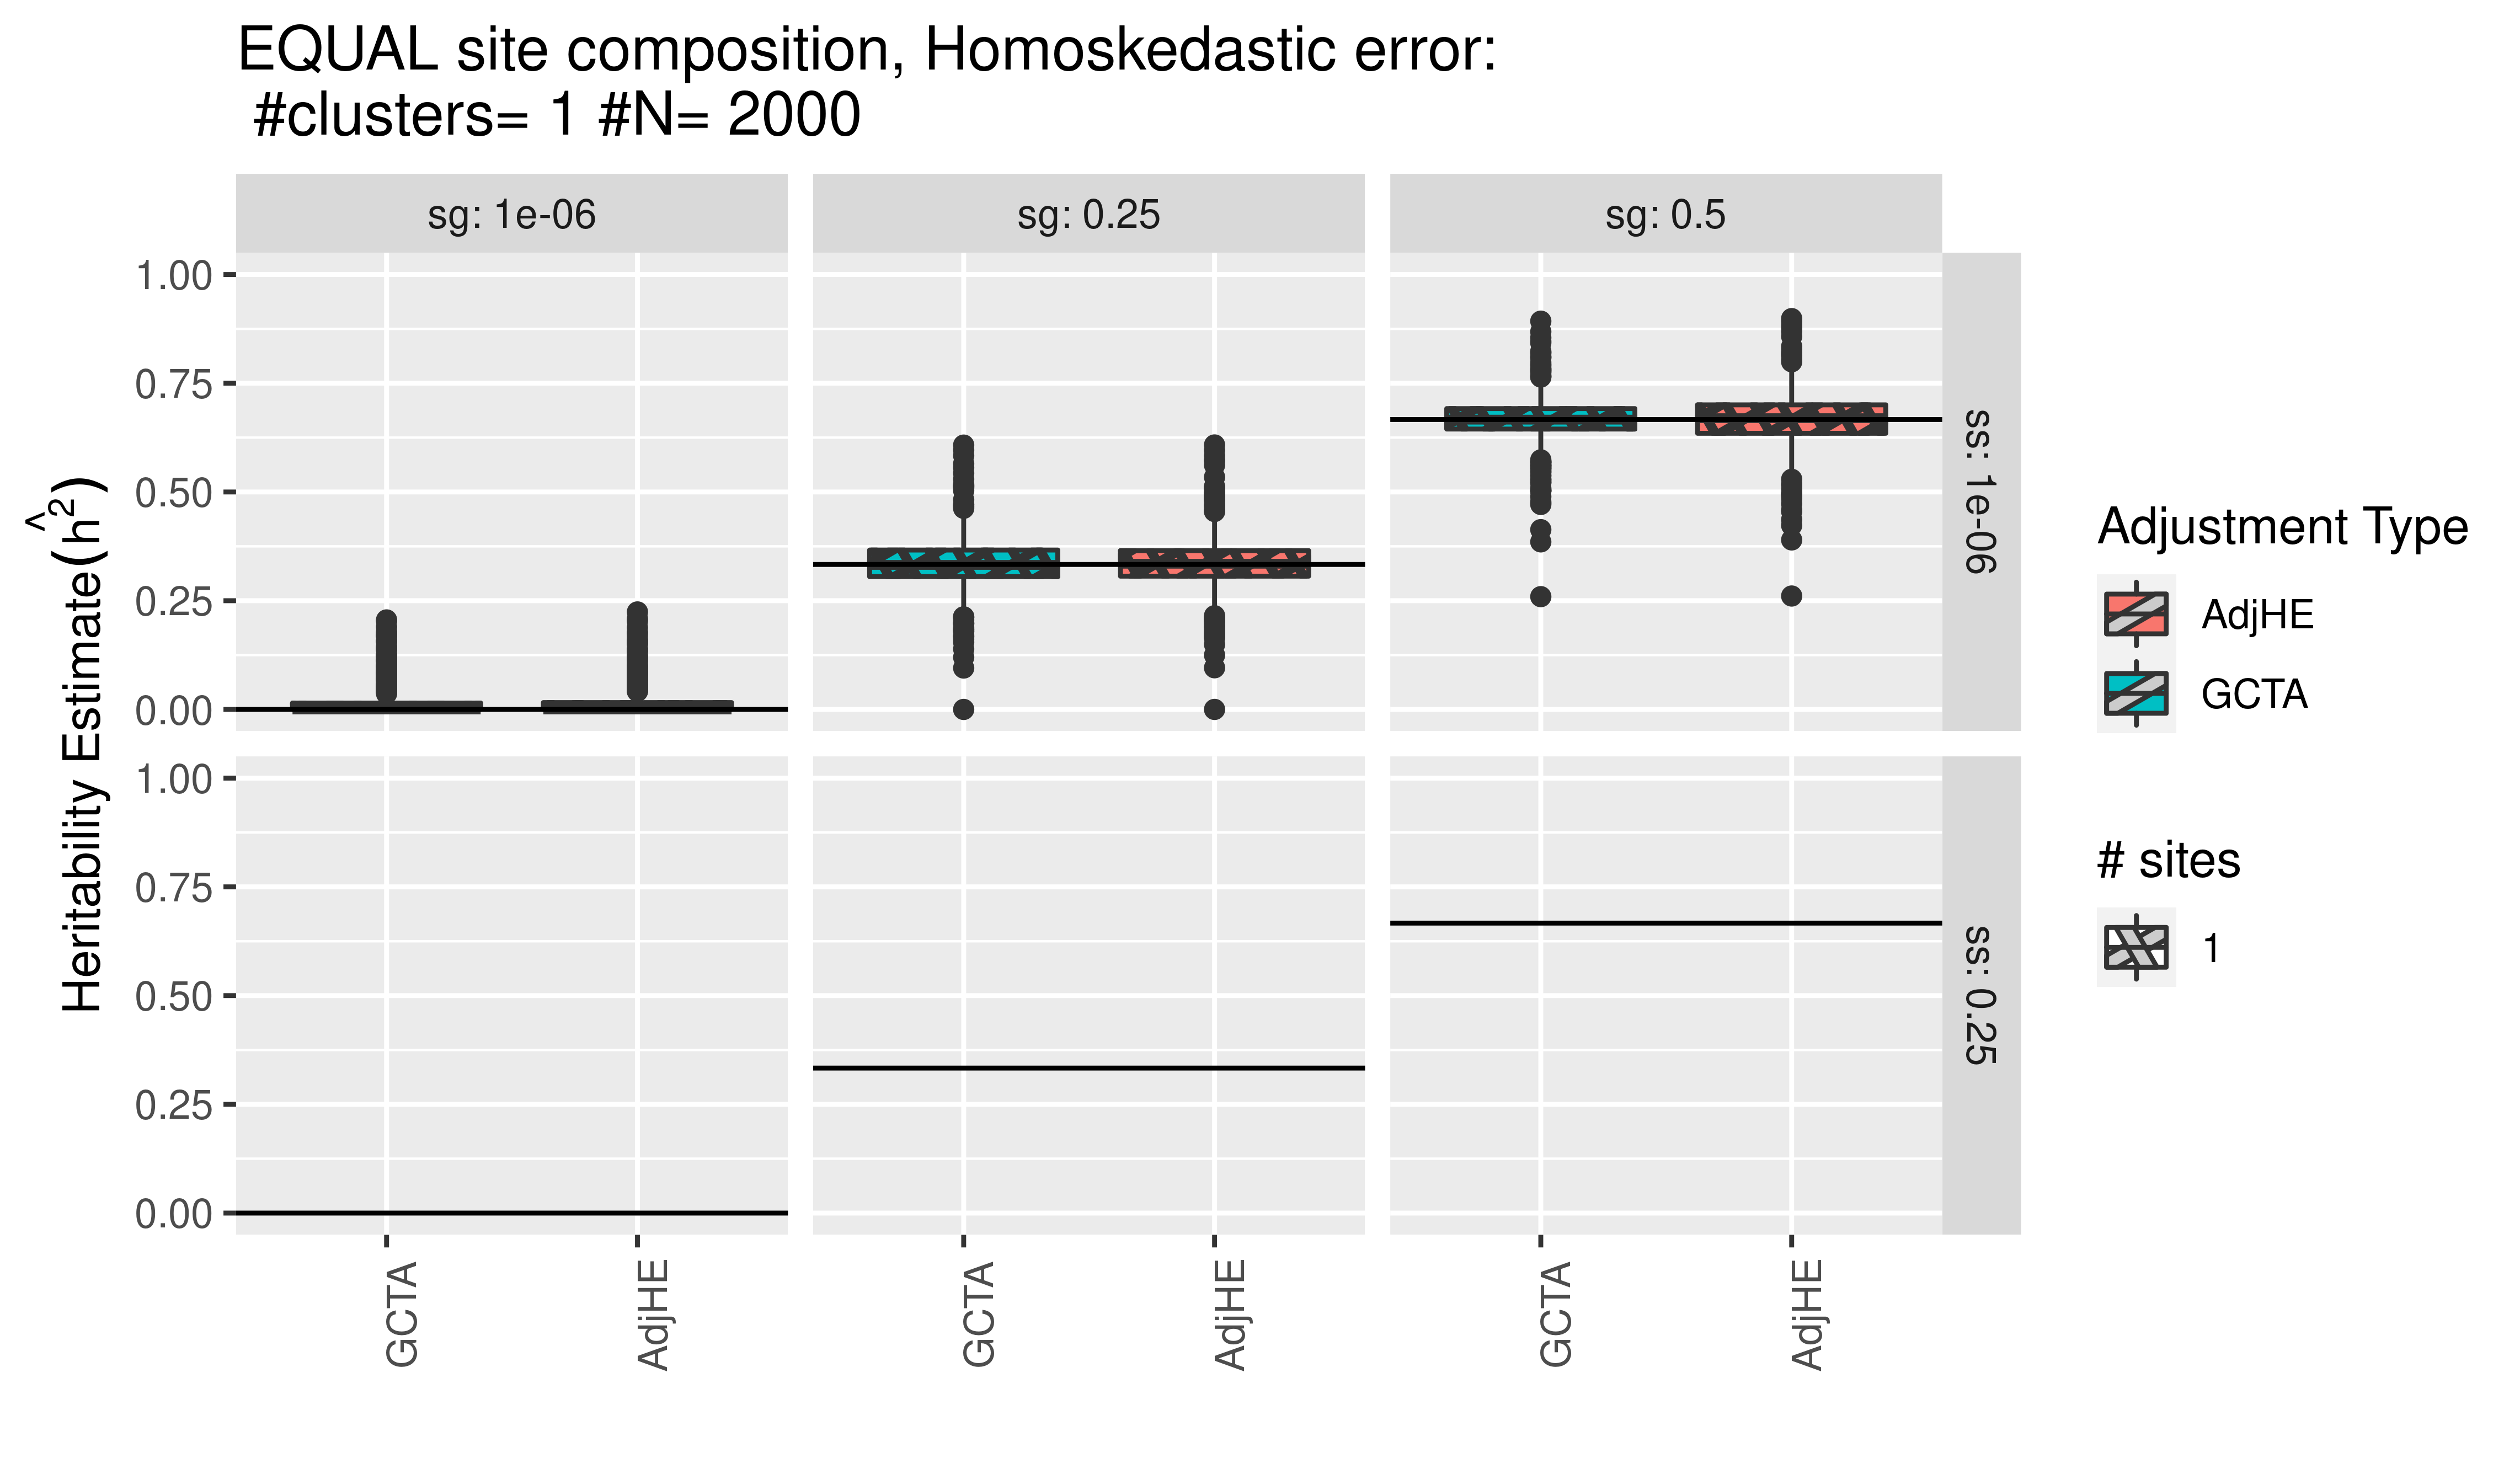
\includegraphics[width = 1.2\textwidth]{/home/christian/Research/Stat_gen/tools/Basu_herit/docs/Figures/Estimates/Simulations/N2000_C1_EQUAL_Homo.png}
\end{frame}


\begin{frame}{Estimation on Homogeneous}
\centering
 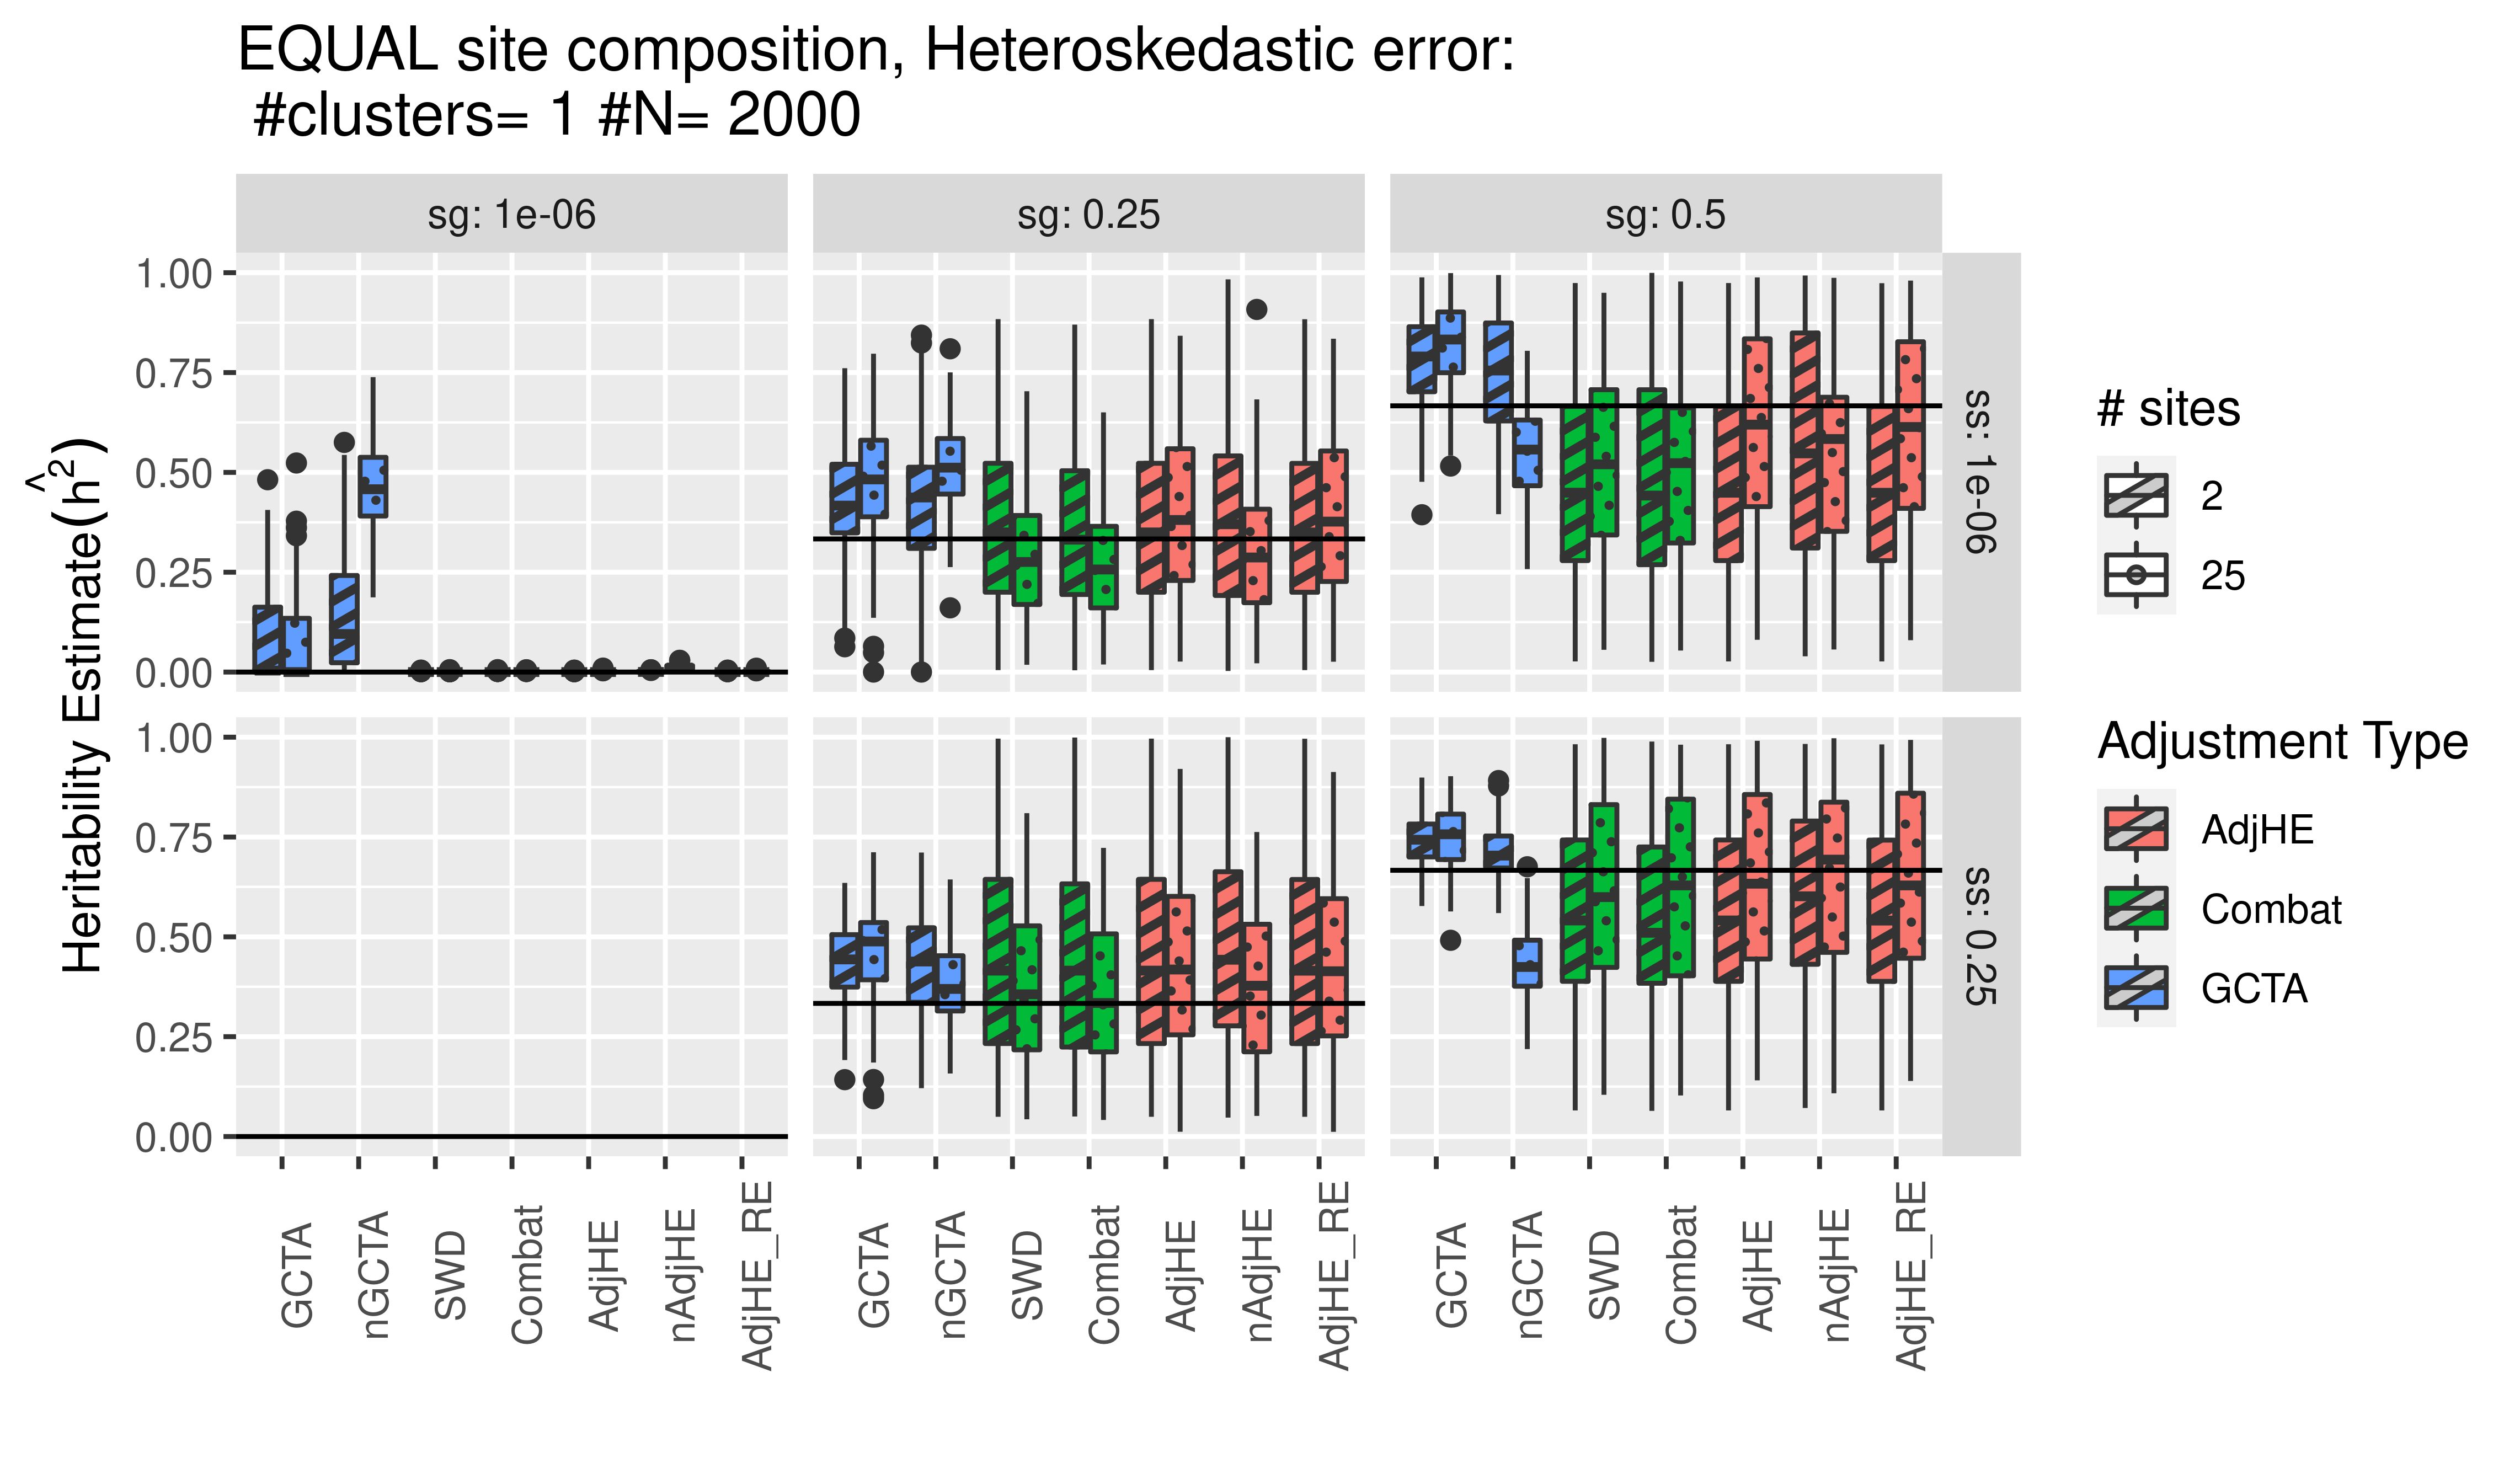
\includegraphics[width = 1.2\textwidth]{/home/christian/Research/Stat_gen/tools/Basu_herit/docs/Figures/Estimates/Simulations/N2000_C1_EQUAL_Het.png}
\end{frame}

\begin{frame}{Multiple clusters heterogeneous}
\centering
 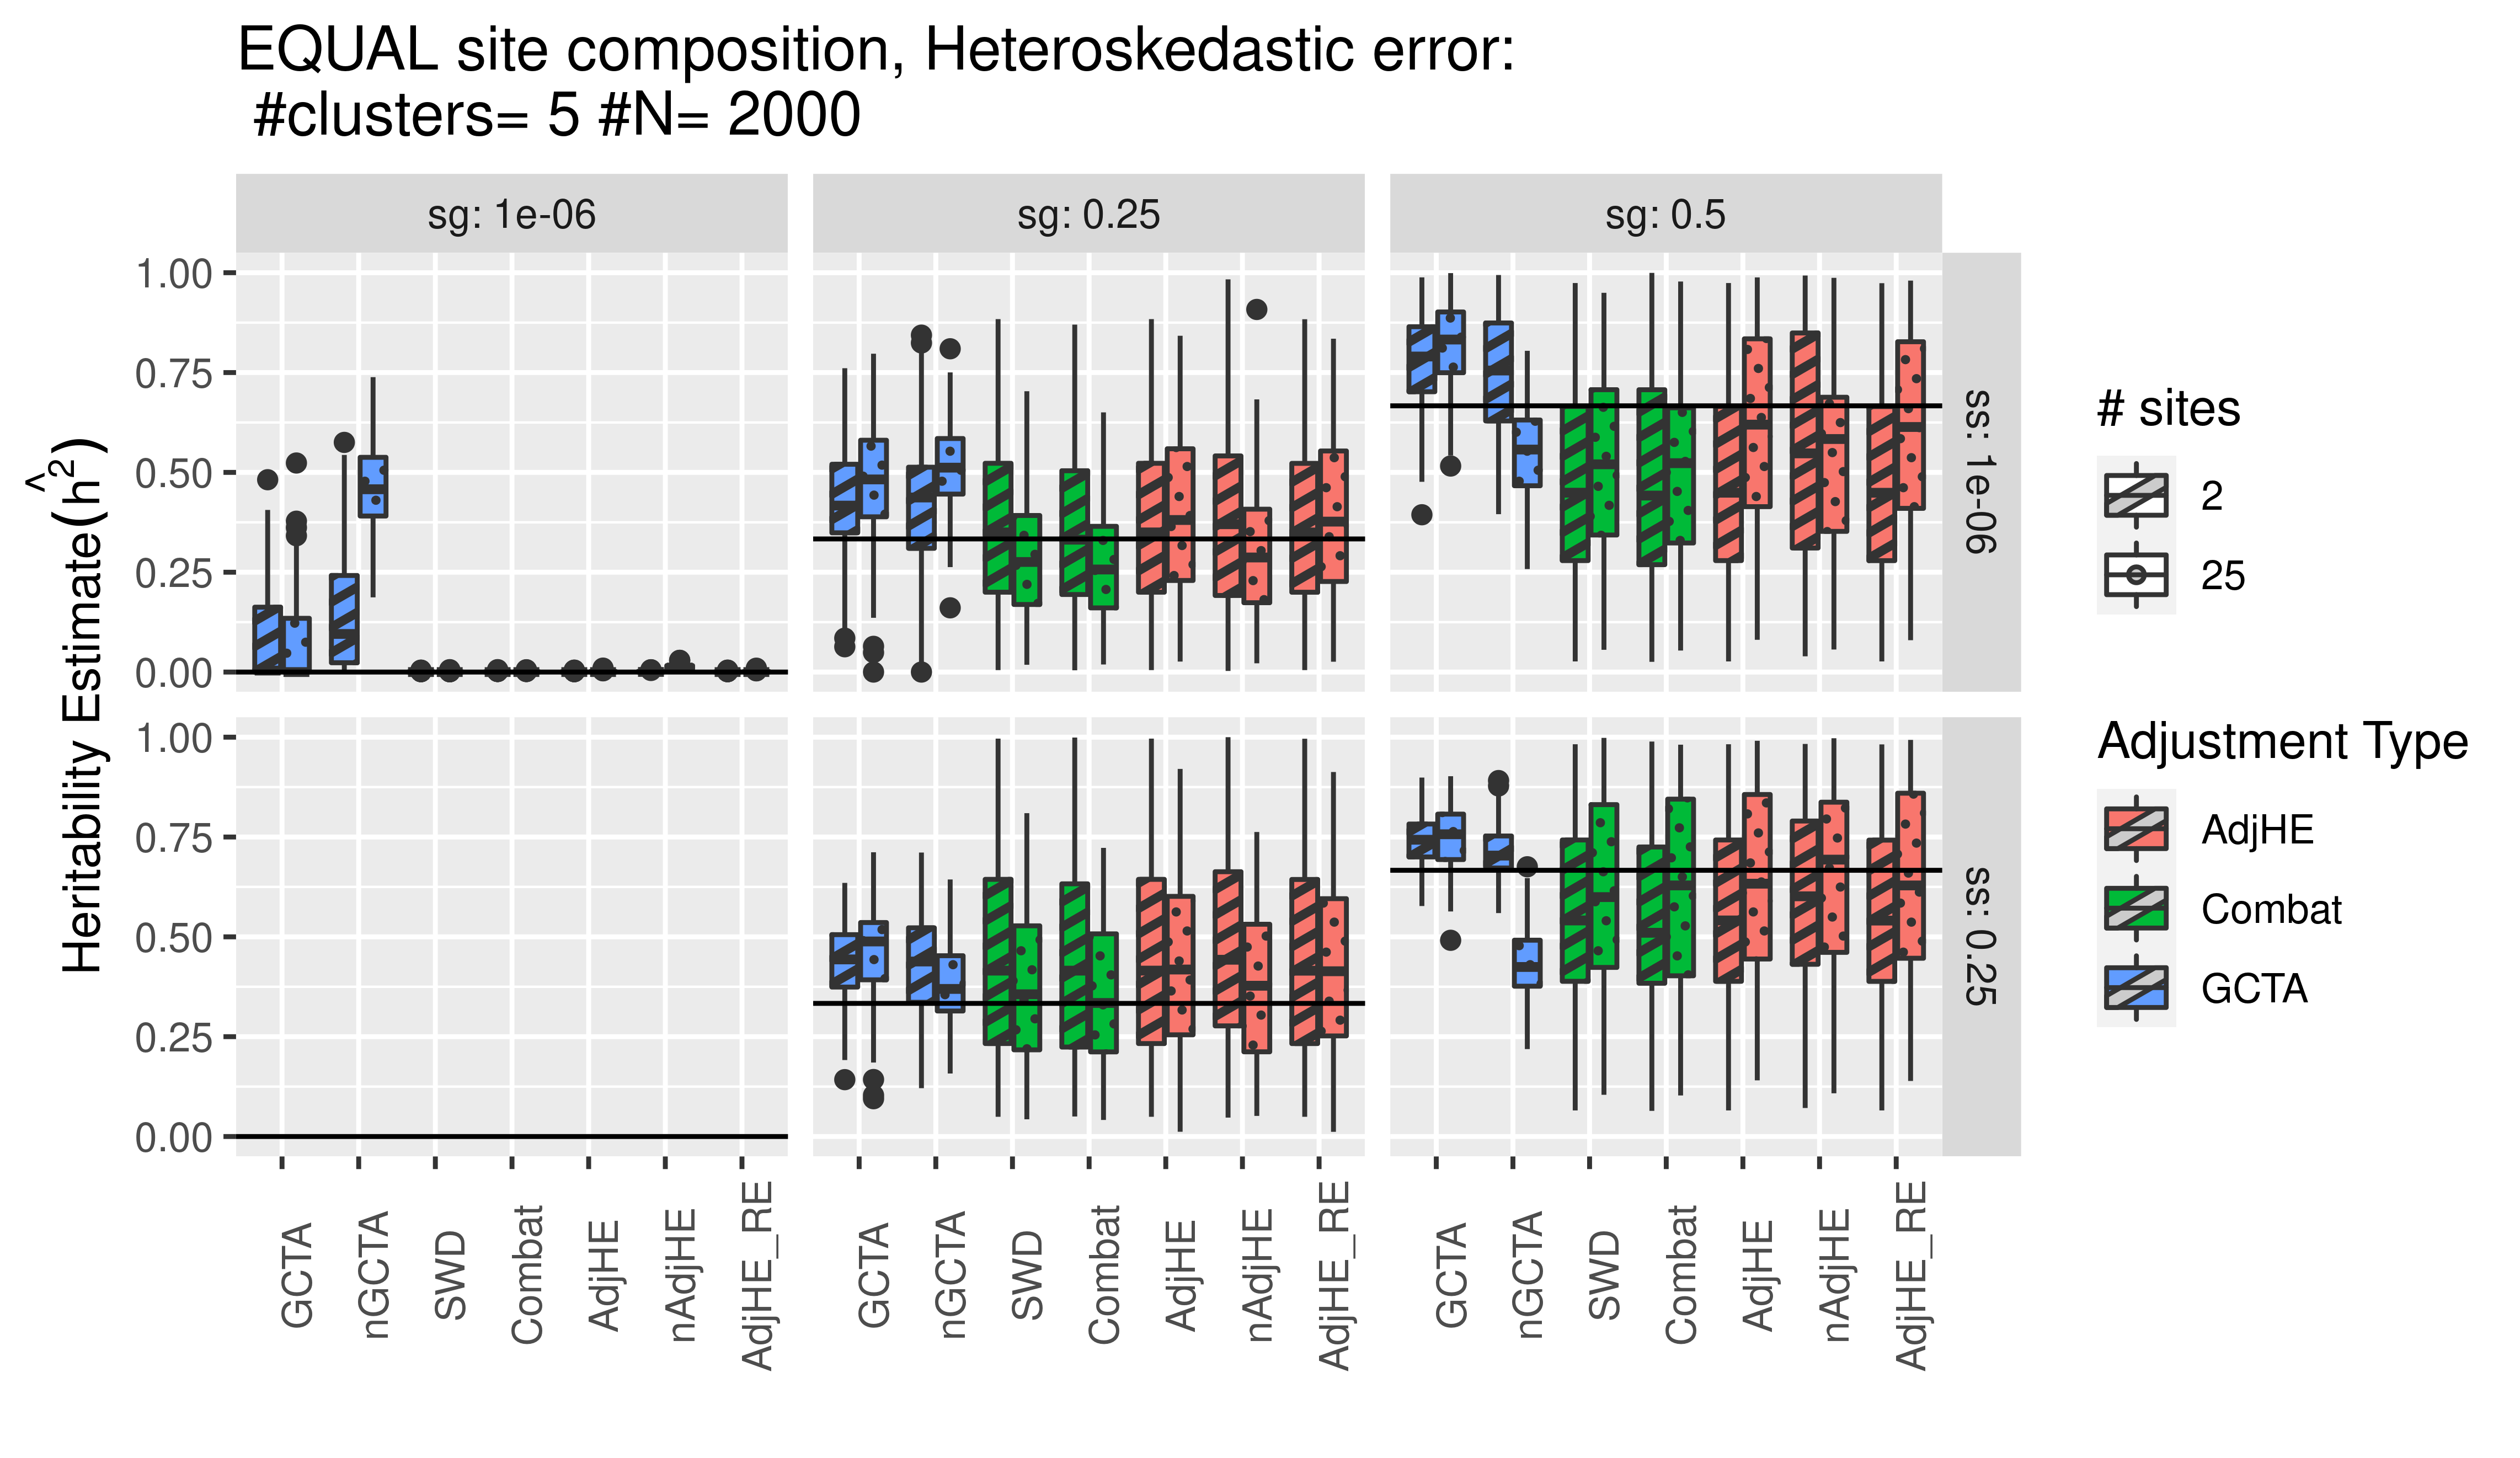
\includegraphics[width = 1.2\textwidth]{/home/christian/Research/Stat_gen/tools/Basu_herit/docs/Figures/Estimates/Simulations/N2000_C5_EQUAL_Het.png}
\end{frame}



\section{Estimation on brain region volumes}
\begin{frame}{Naive estimates on Asegs data}
% 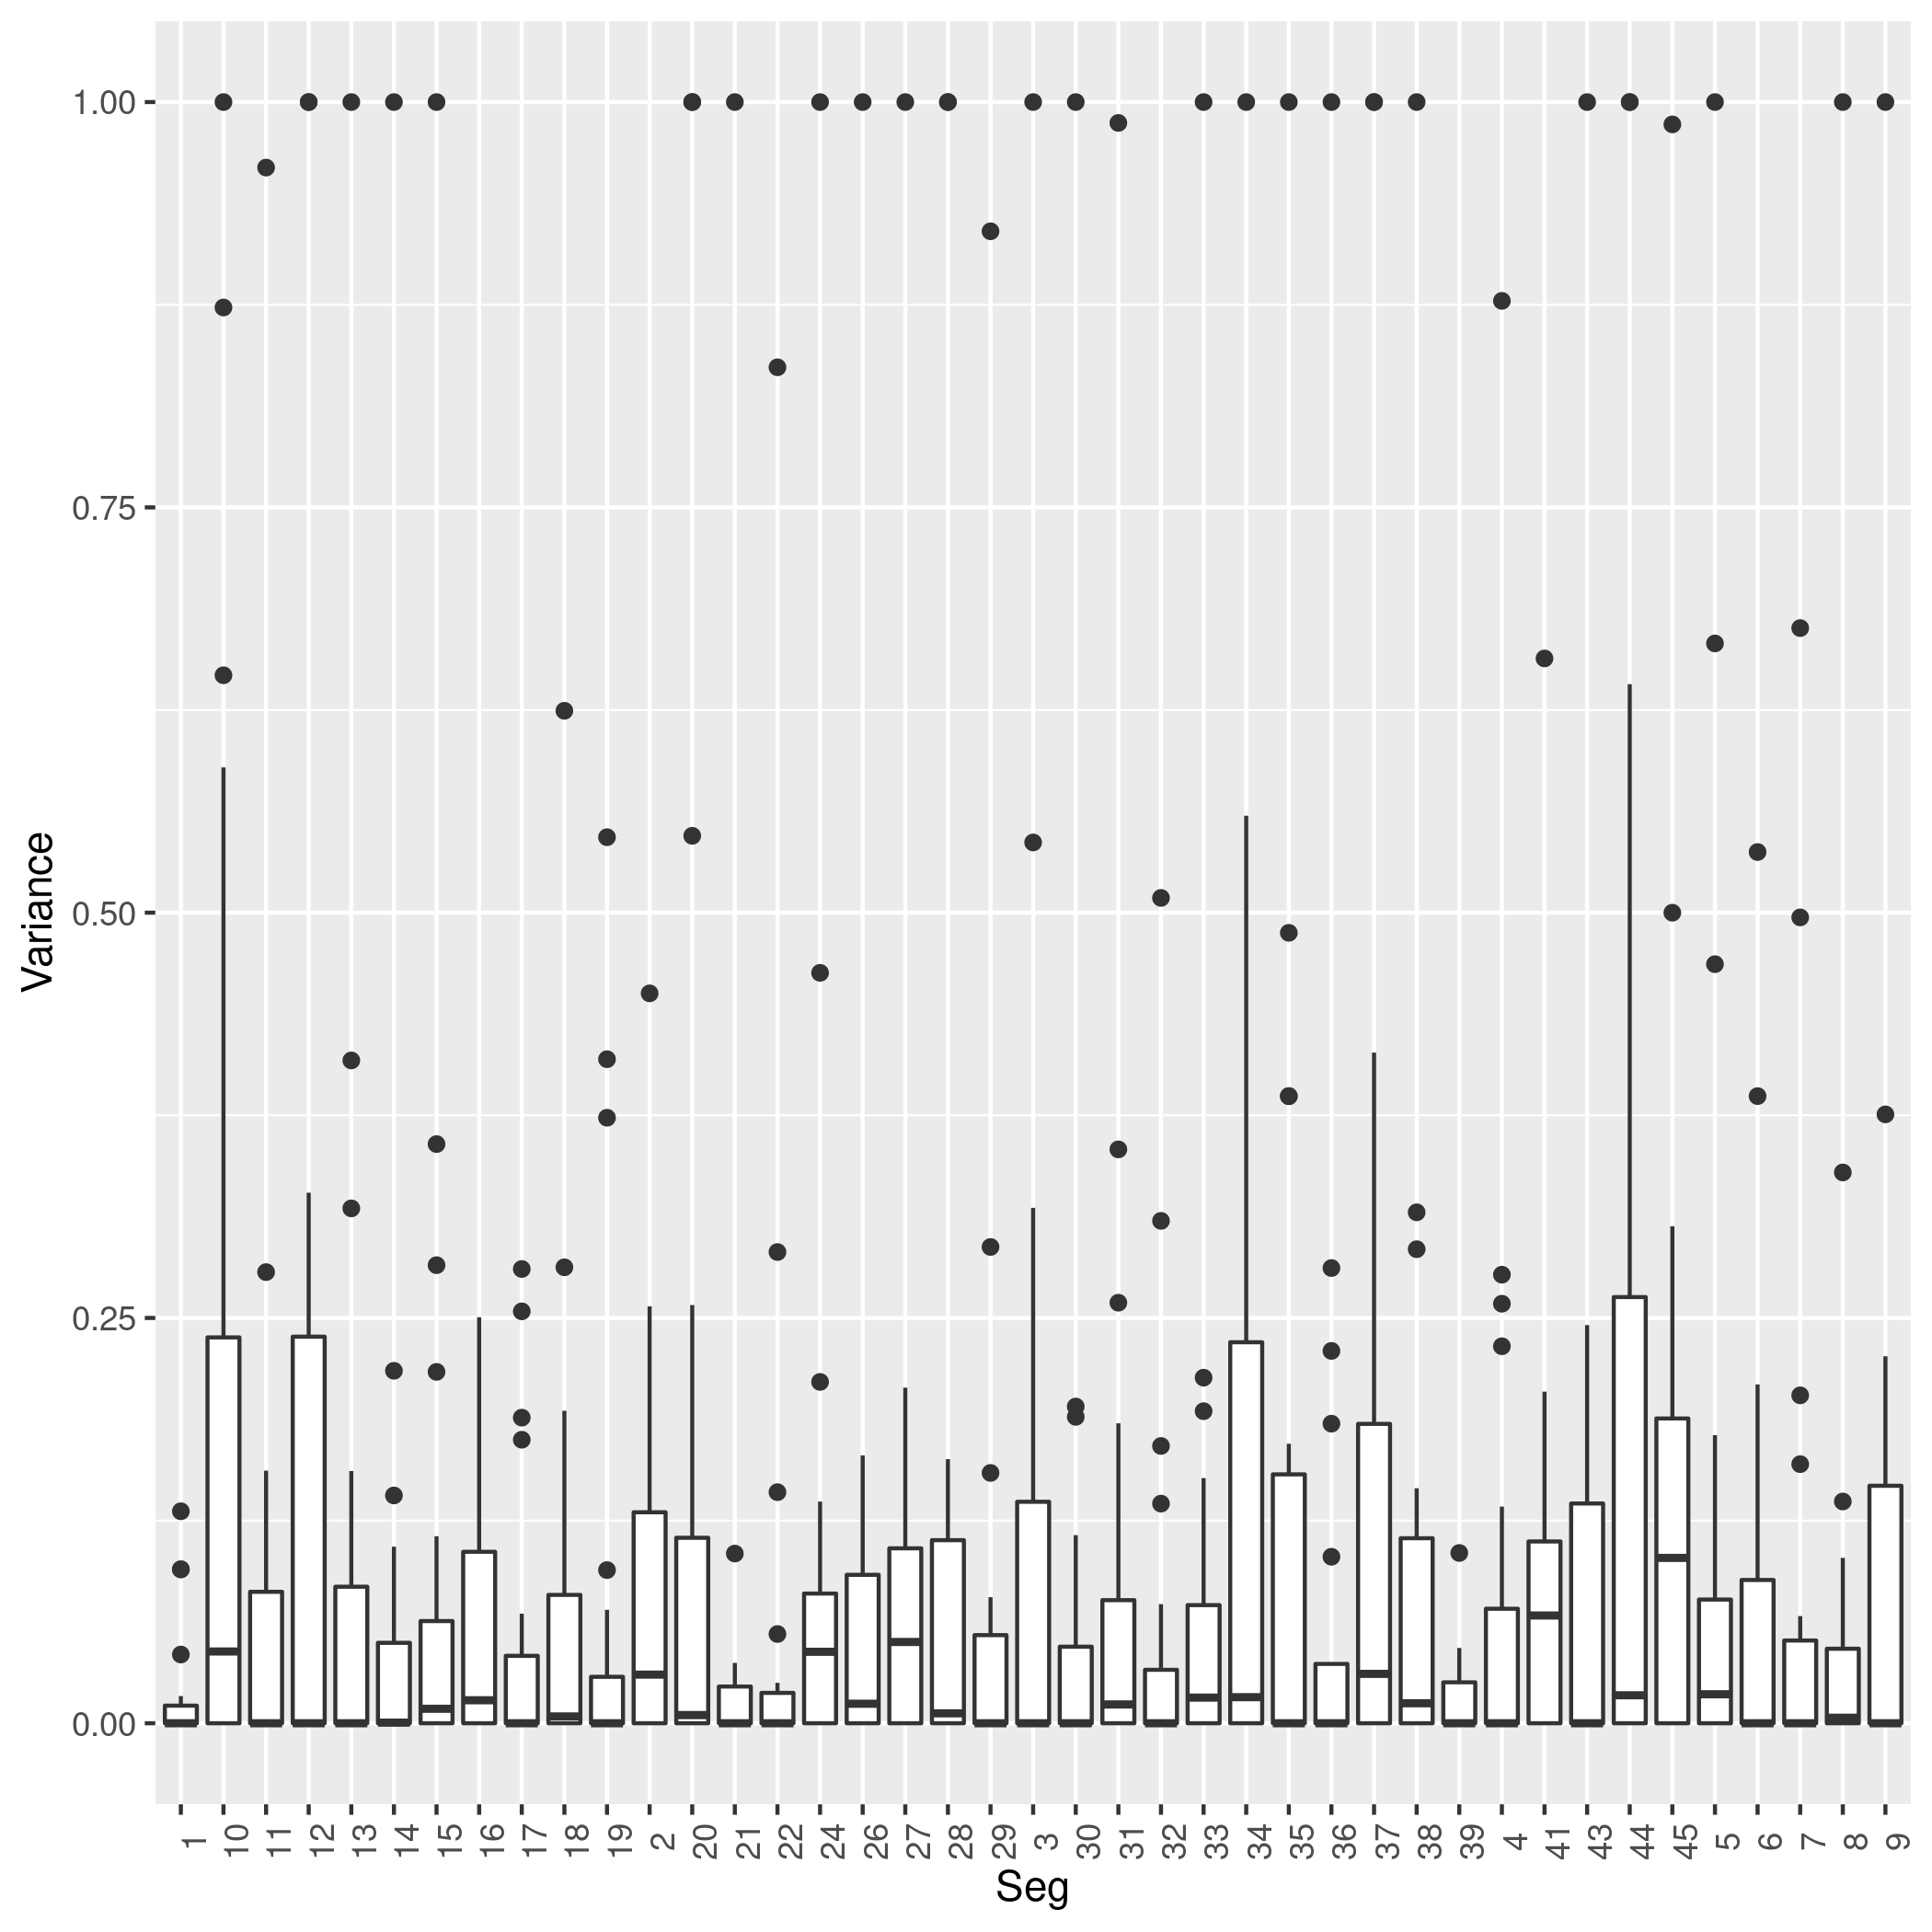
\includegraphics[width = 0.49\textwidth]{/home/christian/Research/Stat_gen/tools/Basu_herit/docs/Figures//naive_GCTA.png}
% 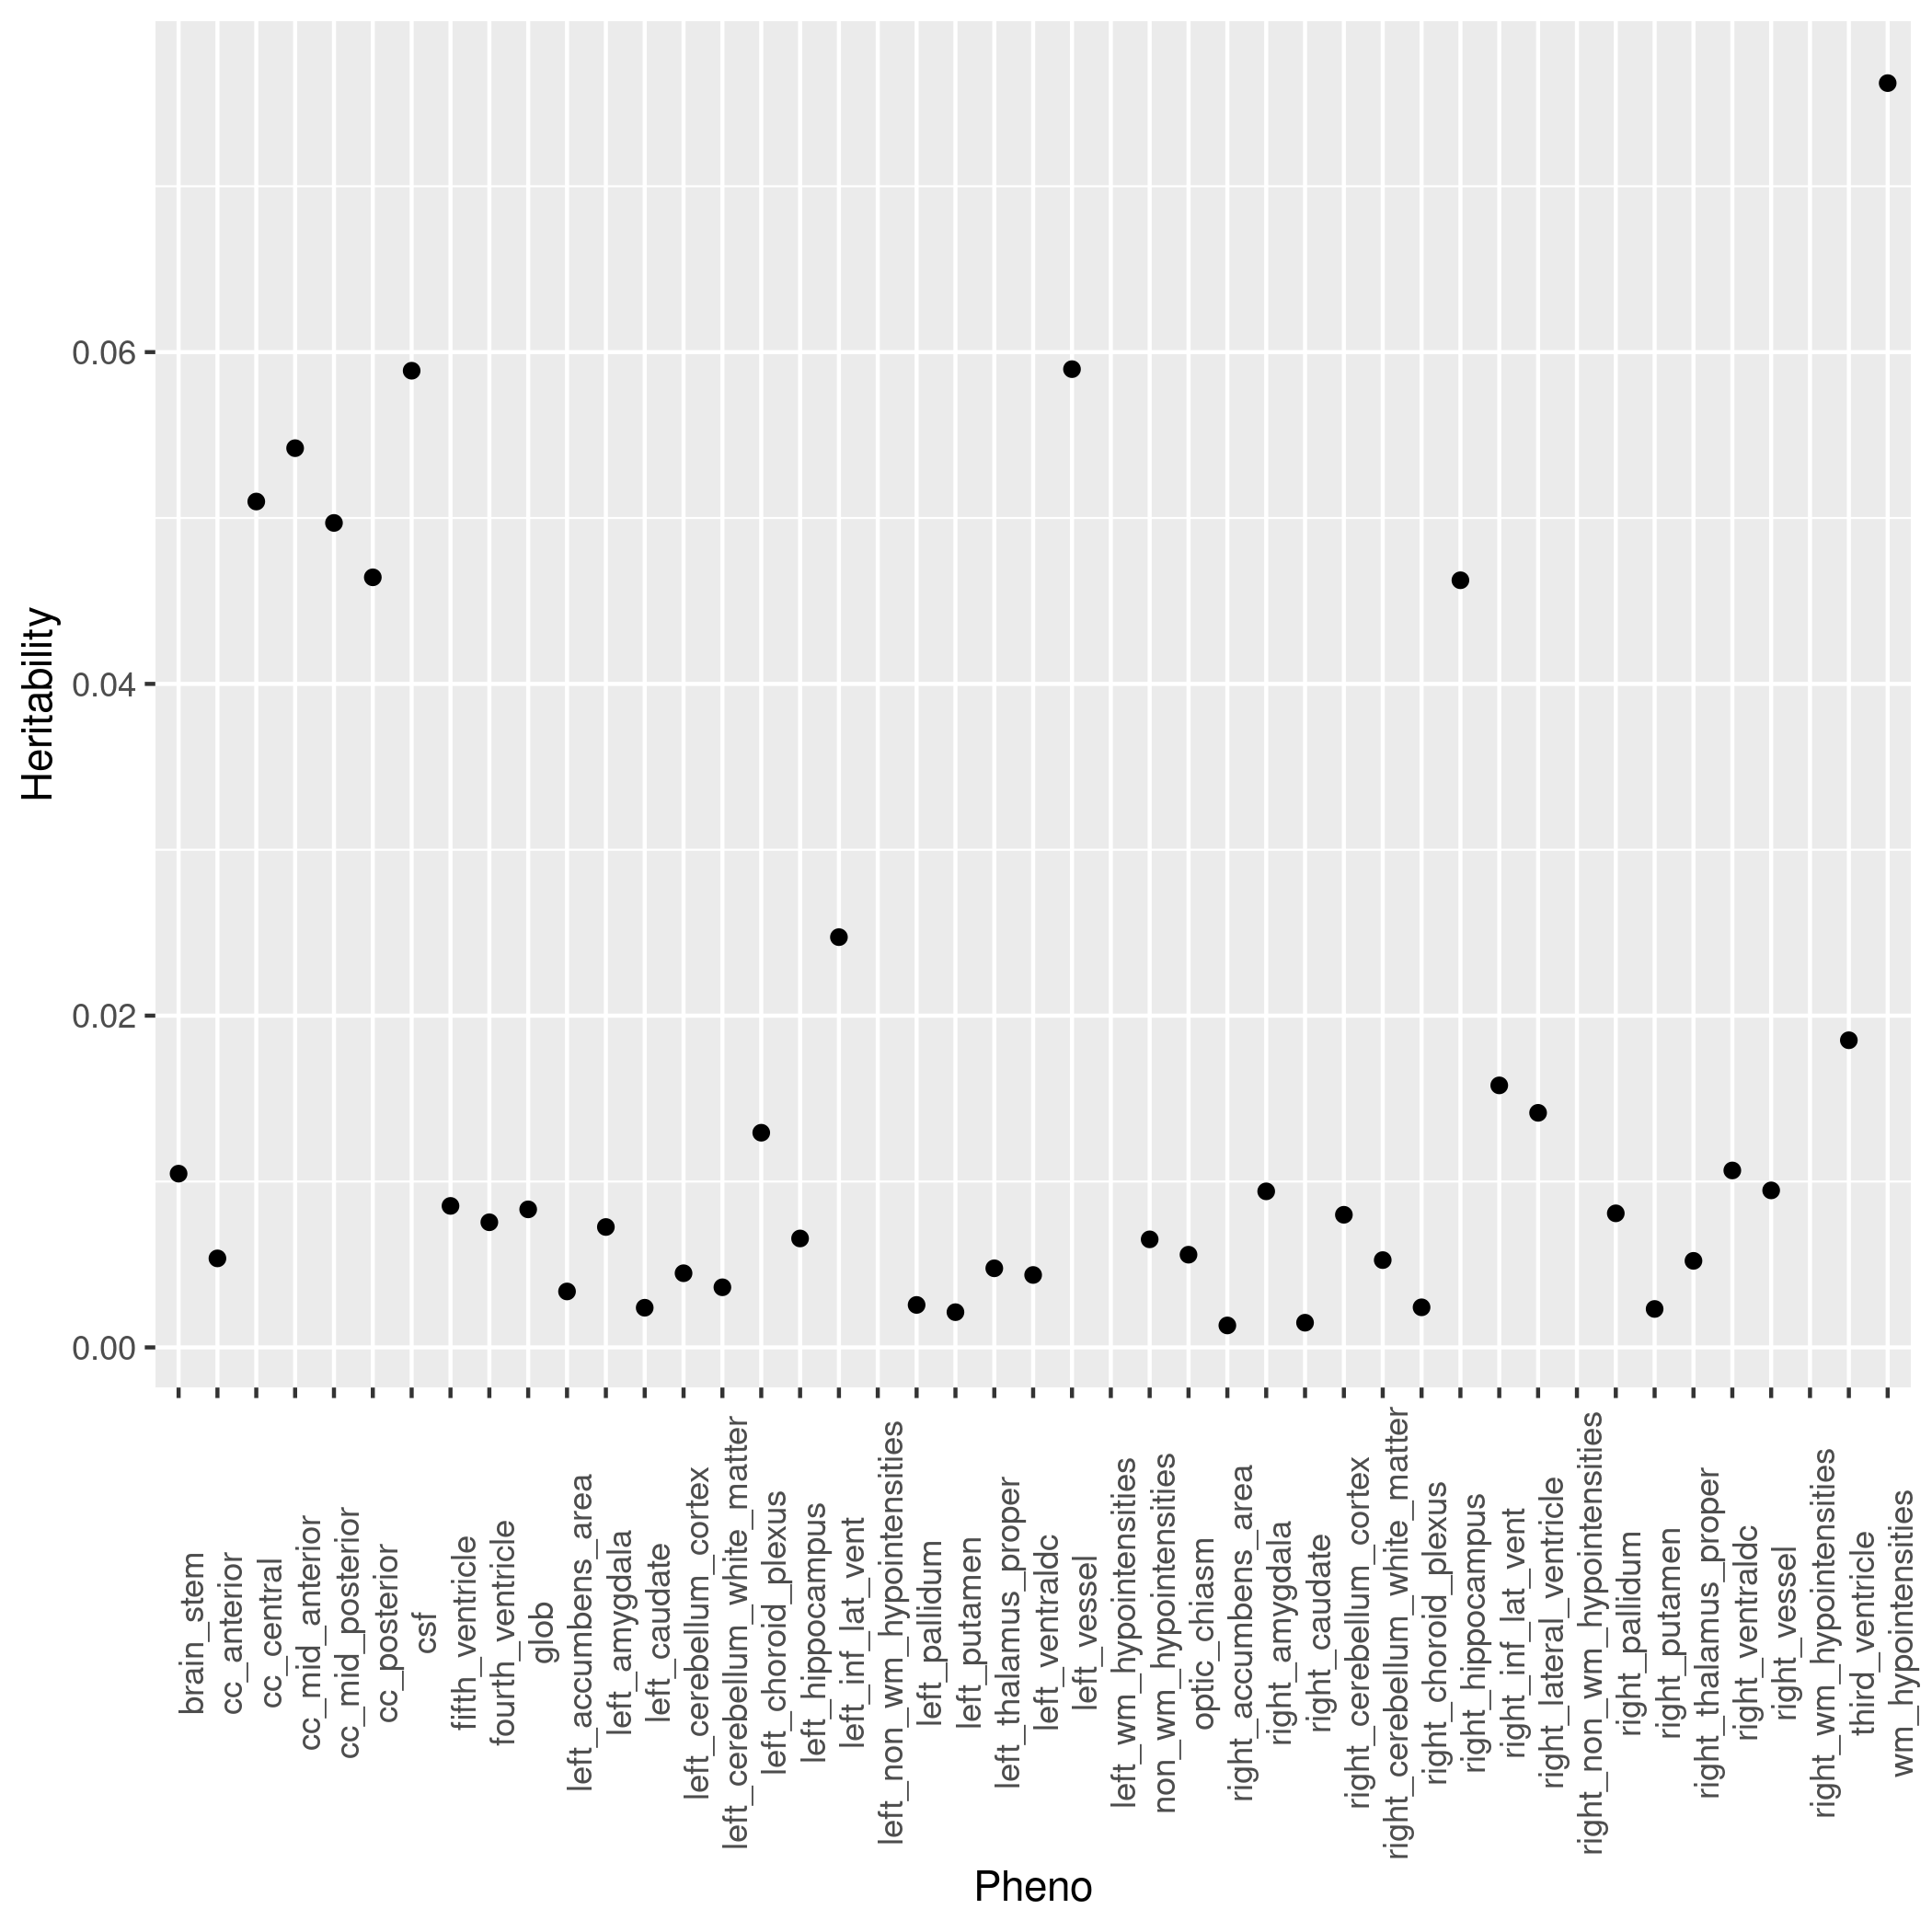
\includegraphics[width = 0.49\textwidth]{/home/christian/Research/Stat_gen/tools/Basu_herit/docs/Presentations/Images/naive_AdjHE.png}
\end{frame}


\begin{frame}{Controlling for Site AdjHE}
% 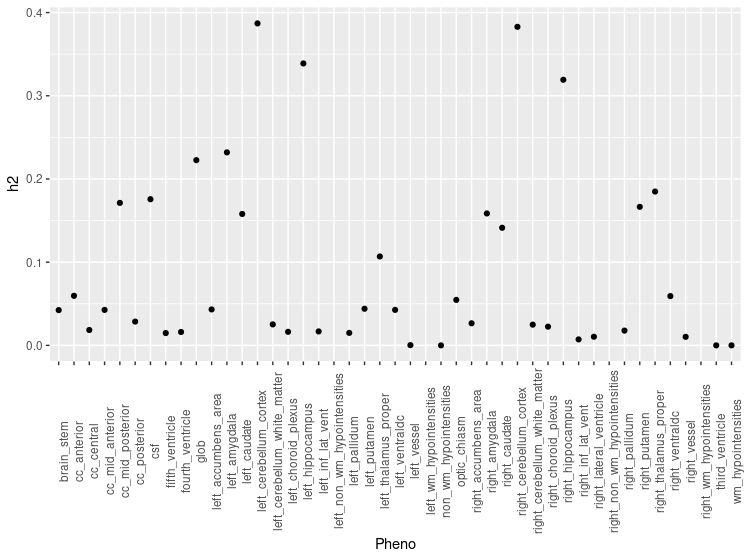
\includegraphics[width = \textwidth]{/home/christian/Research/Stat_gen/tools/Basu_herit/docs/Presentations/Images/Aseg_AdjHE.png}

\end{frame}






\begin{frame}{Conclusions and future aims}
\begin{itemize}
	\item AdjHE is efficient estimator and accounts for basic effect from site
	\item Early analysis suggests volumes in adolescent brains are heritable
	\item Estimates consistent with ADNI results
	\item Applications to functional topology
	\item Differing ethnicity distributions affect estimate?
\end{itemize}
\centering
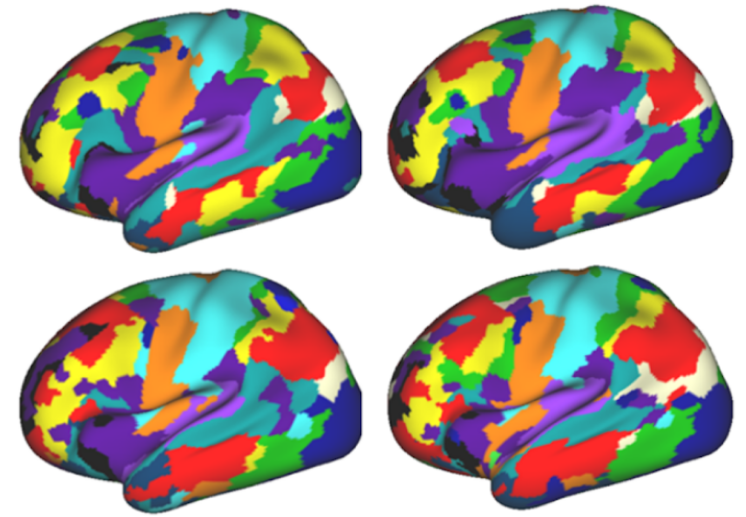
\includegraphics[width = 0.6\textwidth]{/home/christian/Research/Stat_gen/tools/Basu_herit/docs/Figures/Phenotypes/Topologies.png}
\end{frame}


\begin{frame}
\begin{Huge}
Thank you for listening \\
Questions?
\end{Huge}
\end{frame}

\begin{frame}{References}
Lin, Seal, and Basu. “Estimating SNP Heritability in Presence of Population Substructure in Biobank-Scale Datasets.” Genetics 2022 \\
Hermosillo et al. “A Precision Functional Atlas of Network Probabilities and Individual-Specific Network Topography.” 2022 bioRxiv \\
Zhao et al., 2019 “Heritability of Regional Brain Volumes in Large-Scale Neuroimaging and Genetic Studies.”
\end{frame}


\begin{frame}{Source Identifiability problem}
\centering
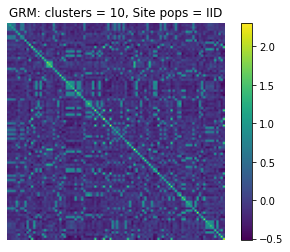
\includegraphics[trim=0cm 0cm 1.8cm 0cm, clip, width = 0.32\textwidth]{/home/christian/Research/Stat_gen/tools/Basu_herit/docs/Figures/Matrices/GRM_mat.png}
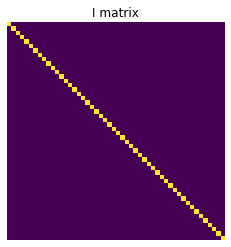
\includegraphics[width = 0.32\textwidth]{/home/christian/Research/Stat_gen/tools/Basu_herit/docs/Figures/Matrices/I_mat.png}
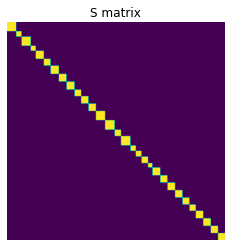
\includegraphics[width = 0.32\textwidth]{/home/christian/Research/Stat_gen/tools/Basu_herit/docs/Figures/Matrices/S_mat.png}
\end{frame}

\begin{frame}{Zhao paper results (ADNI)}
\centering
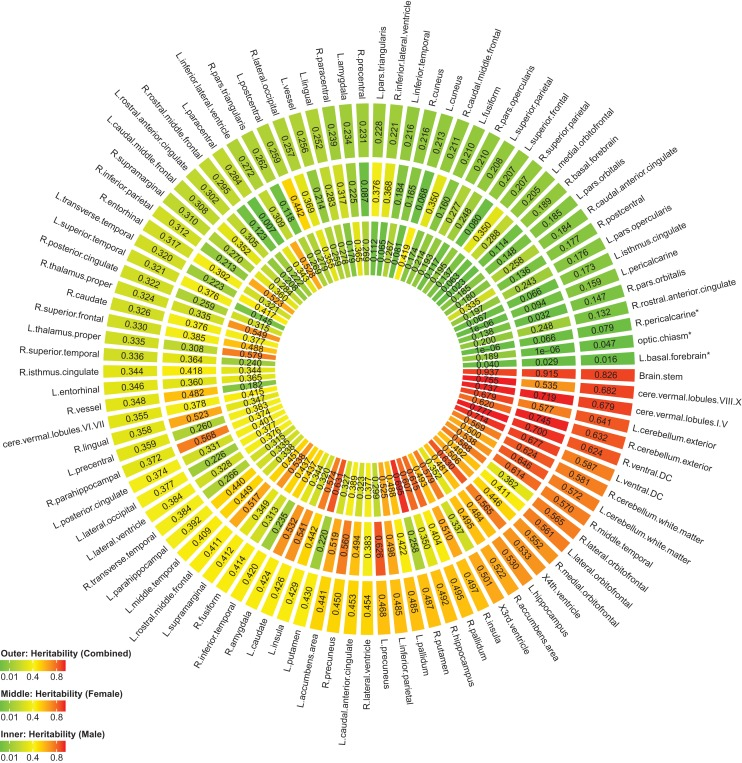
\includegraphics[width =0.8\textwidth]{/home/christian/Research/Stat_gen/tools/Basu_herit/docs/Figures/Estimates/UKB_volume_herits.jpg}
\end{frame}


\end{document}
